% SOURCE_AUTHORITY: sga5_fr_workpass.tex, lines 2610--2744 (LF-normalized unit).
% SOURCE_SHA256: 791F4EFFC5E02832D5D77ED03518C8156D6F07E4C8238B03545DB93D883FBB28
\subsection*{3.6}
En la práctica, es sobre todo la descripción 3.5 b) la que se utiliza. Explicitémosla a nivel de las clases de cohomología, suponiendo, para aligerar la escritura, que $S$ es el espectro de un cuerpo separablemente cerrado. Sea
\[
u\in\Hom_S(L_1,L_2)=\Hom(p_1^*L_1,p_2^!L_2).
\]
Para $x\in\H_c^i(X_1,L_1)$, $u_*(x)\in\H^i(X_2,L_2)$ se define como sigue: se considera el elemento $p_1^*x\in\H^i(X_2,p_{2!}p_1^*L_1)$ deducido de $x$ por imagen inversa, se le aplica $u$, es decir, se forma el producto
\[
u\cdot p_1^*x\in \H^i(X_2,p_{2!}p_2^!L_2),
\]
y luego se aplica la flecha
\[
a:\H^i(X_2,p_{2!}p_2^!L_2)\longrightarrow \H^i(X_2,L_2)
\]
definida por la flecha de adjunción $p_{2!}p_2^!\to\Id$; en resumen:
\begin{equation}
u_*(x)=a(u\cdot p_1^*x).
\tag{3.6.1}
\end{equation}
Sean $c:C\to X$ un morfismo propio y $u\in\Hom(c_1^*L_1,c_2^!L_2)$. Denotemos por
\[
u_*\in\Hom\bigl(R\Gamma_c(X_1,L_1),R\Gamma(X_2,L_2)\bigr)
\]
la imagen de $u$ por la compuesta de 3.2.3 y 3.3.3. De 3.6.1 se deduce que, para $x\in\H_c^i(X_1,L_1)$, se tiene
\begin{equation}
u_*(x)=a(u\cdot c_1^*x),
\tag{3.6.2}
\end{equation}
donde $c_1^*x$ es la imagen inversa de $x$ en $\H^i(X_2,c_{2!}c_1^*L_1)$ y
\[
a:\H^i(X_2,c_{2!}c_2^!L_2)\longrightarrow \H^i(X_2,L_2)
\]
es la flecha deducida de la adjunción $c_{2!}c_2^!L_2\to\Id$. En la situación del ejemplo 3.2 a), se obtiene así
\begin{equation}
\operatorname{cl}(c,N)_*(x)=\mathrm{Tr}_{c_2}(c_1^*x),
\tag{3.6.3}
\end{equation}
donde
\[
\mathrm{Tr}_{c_2}:\H^i(X_2,Rc_{2!}A_C)\longrightarrow\H^{i-2N}(X_2,A(-N))
\]
es la flecha inducida por el morfismo de traza relativo a $c_2$. Esta fórmula concuerda, para $N=0$, con (SGA $4^{1/2}$ Ciclo 3.6): $\operatorname{cl}(c)_*$ es el homomorfismo denotado por $\eta_{X_2,X_1}$ en (loc. cit.). Si $X_1$ es liso, de dimensión relativa pura $r_1$, y $c$ es una inmersión cerrada, de 3.6.1 y de la observación hecha al final de 3.2 a) se deduce que también se tiene
\begin{equation}
\operatorname{cl}(c,N)_*(x)=\mathrm{Tr}_{p_2}(\operatorname{cl}(C)\,p_1^*x),
\tag{3.6.4}
\end{equation}
donde $\operatorname{cl}(C)\in \H_C^{2(r_1-N)}(X,A(r_1-N))$ es la clase de cohomología de $C$ y
\[
\mathrm{Tr}_{p_2}:\H^*(X_2,Rp_{2!}A_X)\longrightarrow \H^{*-2r_1}(X_2,A(-r_1))
\]
es la flecha definida por el morfismo de traza relativo a $p_2$. Se recupera la definición habitual del homomorfismo inducido en la cohomología por una correspondencia ([12] 1.3), (SGA $4^{1/2}$ Ciclo 3.2).

\subsection*{3.6.5}
En la situación de 3.2 b), de 3.6.2 se deduce que, para $u\in\Hom(F^*L_1,L_2)$,
\[
u_*:\H_c^i(X_1,L_1)\longrightarrow \H^i(X_2,L_2)
\]
es la compuesta del homomorfismo ``imagen inversa''
\[
\H_c^i(X_1,L_1)\longrightarrow \H^i(X_2,F^*L_1)
\]
y del homomorfismo inducido por $u$ (más generalmente, $f_*u:Rf_{1!}L_1\to Rf_{2*}L_2$ es la compuesta del homomorfismo canónico
\[
Rf_{1!}L_1\longrightarrow Rf_{2*}F^*L_1
\]
y de $Rf_{2*}u$). En particular, la correspondencia diagonal induce la flecha canónica
\[
Rf_{1!}L_1\longrightarrow Rf_{1*}L_1
\]
(la identidad si $X_1$ es propio sobre $S$).

\subsection*{3.7}
Volvamos a la situación del comienzo de 3.3, suponiendo dado además un cuadrado conmutativo
\begin{equation}
\begin{tikzcd}[column sep=3em,row sep=2em]
X \arrow[d,"f"'] & C \arrow[l,"c"'] \arrow[d,"g"] \\
Y & D \arrow[l,"d"]
\end{tikzcd}
\tag{3.7.1}
\end{equation}
con $c$ propio. Pongamos $c_i=p_ic$, $d_i=q_id$, donde $p_i:X\to X_i$, $q_i:Y\to Y_i$ son las proyecciones. De 3.7.1 se deduce un diagrama conmutativo en el que el cuadrado interior es cartesiano:
\begin{equation}
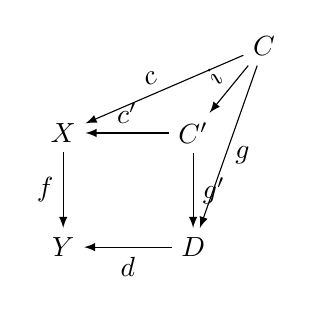
\begin{tikzpicture}[>=latex,baseline=(current bounding box.center),scale=1]
\node (X) at (0,0) {$X$};
\node (Y) at (0,-1.45) {$Y$};
\node (Cp) at (1.65,0) {$C'$};
\node (D) at (1.65,-1.45) {$D$};
\node (C) at (2.55,1.1) {$C$};
\draw[->] (C) -- node[above,sloped,pos=.55] {$c$} (X);
\draw[->] (C) -- node[above,sloped,pos=.50] {$i$} (Cp);
\draw[->] (C) -- node[right,pos=.55] {$g$} (D);
\draw[->] (Cp) -- node[above] {$c'$} (X);
\draw[->] (Cp) -- node[right] {$g'$} (D);
\draw[->] (X) -- node[left] {$f$} (Y);
\draw[->] (D) -- node[below] {$d$} (Y);
\end{tikzpicture}
\tag{3.7.2}
\end{equation}
Para $K\in\ob\Dctf(X)$, se tiene una flecha canónica
\begin{equation}
f_*c_*c^!K\longrightarrow d_*d^!f_*K,
\tag{3.7.3}
\end{equation}
compuesta de la flecha
\[
f_*c_*c^!K=f_*c'_*(i_*i^!)c'^!K\longrightarrow f_*c'_*c'^!K=d_*g'_*c'^!K
\]
definida por la flecha de adjunción $i_*i^!\to\Id$, y del isomorfismo
\[
d_*g'_*c'^!K\xrightarrow{\sim}d_*d^!f_*K
\]
definido por el isomorfismo canónico $g'_*c'^!\xrightarrow{\sim}d^!f_*$ (SGA 4 XVIII 3.1.12.3). Tomando $K=\uRHom_S(L_1,L_2)$, y componiendo 3.7.3 con el isomorfismo deducido de 3.3.1, se obtiene una flecha canónica
\begin{equation}
f_*c_*c^!\uRHom_S(L_1,L_2)
\longrightarrow
 d_*d^!\uRHom_S(f_{1!}L_1,f_{2*}L_2),
\tag{3.7.4}
\end{equation}
que, gracias a 3.2.1, puede reescribirse
\begin{equation}
f_*c_*\uRHom(c_1^*L_1,c_2^!L_2)
\longrightarrow
 d_*\uRHom(d_1^*(f_{1!}L_1),d_2^!(f_{2*}L_2)).
\tag{3.7.5}
\end{equation}
De ella se deduce
\begin{equation}
f_*:\Hom(c_1^*L_1,c_2^!L_2)
\longrightarrow
\Hom(d_1^*(f_{1!}L_1),d_2^!(f_{2*}L_2)).
\tag{3.7.6}
\end{equation}
La flecha 3.7.5 (resp. 3.7.6) generaliza 3.3.1 (resp. 3.3.2), con la cual coincide cuando $c$ y $d$ son las identidades. Nótese también que, para $c$ propio, 3.2.2 (resp. 3.2.3) no es sino 3.7.5 (resp. 3.7.6) cuando $f_1$, $f_2$ y $d$ son las flechas identidad. Cuando $Y_1=Y_2=S=D$, abreviaremos $f_*u$ como $u_*$, como antes.

\section{Apareamientos de correspondencias. Fórmula de Lefschetz}
